%%=============================================================================
%% Methodologie
%%=============================================================================

\chapter{\IfLanguageName{dutch}{proof-of-concept}{proof-of-concept}}%
\label{ch:proof-of-concept}

Dit hoofdstuk omvat de proof of concept van dit onderzoek. Een van de game-engines die in de short-list zit is Godot. Met deze engine zal er een proof of concept geïmplementeerd worden.

\section{Doelstelling}
De proof of concept heeft als doelstelling een space-invaders videospel te implementeren in Godot met gebruik makend van C\# als de scripttaal voor de engine. Hierdoor weet Allphi of het mogelijk is en zouden ze het kunnen recreëren.

\section{Implementatie}
Het spel is ontwikkeld in Godot gebruikmakend van C\# als de scripttaal. Het is mogenlijk om in Godot hun eigen taal genaamd GDScript te gebruiken. Het gebruik van C\# is niet ondersteund in de script editor van Godot. Hierdoor moet je een apparte versie van Godot installeren. Eenmaal dat de engine is geinstalleerd kan je deze openen. In de instelling moet je dan selecteren welke IDE je wilt gebruiken voor het schrijven van de scripts. Hiervoor kies je het best Visual Studio. Er wordt dan een solution aangemaakt in je project waardoor je een de voordelen van C\# te gebruiken hebt. Godot heeft een goede documentatie die zowel hun eigen script als C\# ondersteund. Je kan bij de meeste stukken code verwisselen van taal.

\begin{figure}[h]
    \centering
    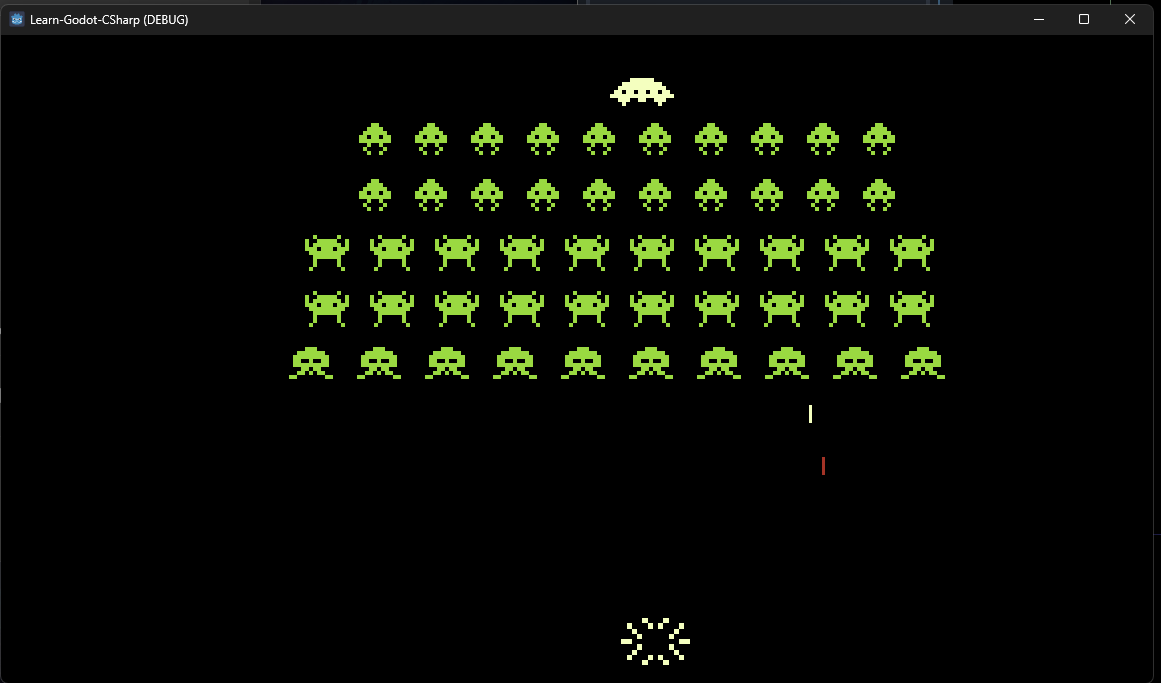
\includegraphics[width=1\textwidth]{ImplementatieSpel.png}
    \caption{Implementatie}
    \label{fig:POC}
\end{figure}

\section{Conclusie}
